% BRED

\section{Introduction}

One of the central cellular processes underlying development is transcriptional regulation. During development, changes in transcription factor activity induce chromatin modifications, chromatin remodelling and ultimately a differential recruitment of the basal transcriptional machinery\cite{coulon_eukaryotictranscriptionaldynamics_2013}. Modelling the dynamics of gene regulation is therefore essential to better understand why a cellular dynamic processes progresses through several steps, and what goes wrong in the case of disease.

The dynamics of gene regulation has classically been studied using time series data\cite{bar-joseph_studyingmodellingdynamic_2012}. When dynamic processes progress asynchronously, such as in hematopoiesis, time series data are usually obtained by sorting different transition states and assessing bulk gene expression and transcription factor binding within the population\cite{novershtern_denselyinterconnectedtranscriptional_2011, may_dynamicanalysisgene_2013, jojic_identificationtranscriptionalregulators_2013, goode_dynamicgeneregulatory_2016}. Alternatively, time series data can also be generated by synchronizing the dynamic process between cells. However, issues with time-resolution, heterogeneity and good in vivo synchronization models can often limit the predictive power of the dynamic models of gene regulation which can be constructed\cite{bar-joseph_studyingmodellingdynamic_2012}.

One of the main advantages of single-cell transcriptomics is the ability to quantify the exact cellular state of thousands of cells per experiment. The intercellular heterogeneity caused by naturally occurring biological stochasticity \cite{padovan-merhar_usingvariabilitygene_2013} can be exploited to predict regulatory interactions between transcription factors (TFs) and their target genes. The computational tools that infer gene regulatory networks (GRNs) from omics datasets are called network inference (NI) methods.
% TODO: talk about bulk NI

Several studies have highlighted how some regulatory interactions can be very dynamic while others show evidence of being static during consecutive developmental stages\cite{moignard_characterizationtranscriptionalnetworks_2013, pina_singlecellnetworkanalysis_2015}. 
Since regulatory interactions are context-dependent\cite{papp_genomewideanalysiscontextdependence_2005}, attempting to create an accurate model of those processes by inferring a static regulatory network may have limited relevance.

Case-specific NI (CSNI) methods avoid predicting a global GRN and instead produce one GRN per case in the dataset.
The sample-specific GRNs -- or 'sample-specific regulomes' -- can be used in much the same way as single-cell transcriptomi

 Kuijjer et al.\cite{kuijjer_estimatingsamplespecificregulatory_2019} LOO. Liu et al. \cite{personalizedcharacterizationdiseases}. Aibar et al. SCENIC \cite{aibar_scenicsinglecellregulatory_2017} use global method and post-process.




NI methods that take into account the dynamic aspect of gene regulation instead produce network models with variable regulatory activity.

 To this end, several approaches have been proposed, which can be broadly classified in three different classes, depending on the output structure they produce: differential NI, dynamic NI, and profile-specific NI (Figure \ref{fig:ni_types}). 

With each of these methodologies, it should be noted that while they produce networks specific for only certain subsets of the cell's profiles, they still use the information from all available profiles. 
If a method is to infer a network from cells in only a certain condition, it will infer interactions from noise in the data, rather than the changes that separate that condition from any other.
As such, a context-dependent network inferred from only a subset of the profiles is likely to be less accurate than a static network trained on all profiles.



\section{Results}

\begin{figure}[htb!]
	\centering
	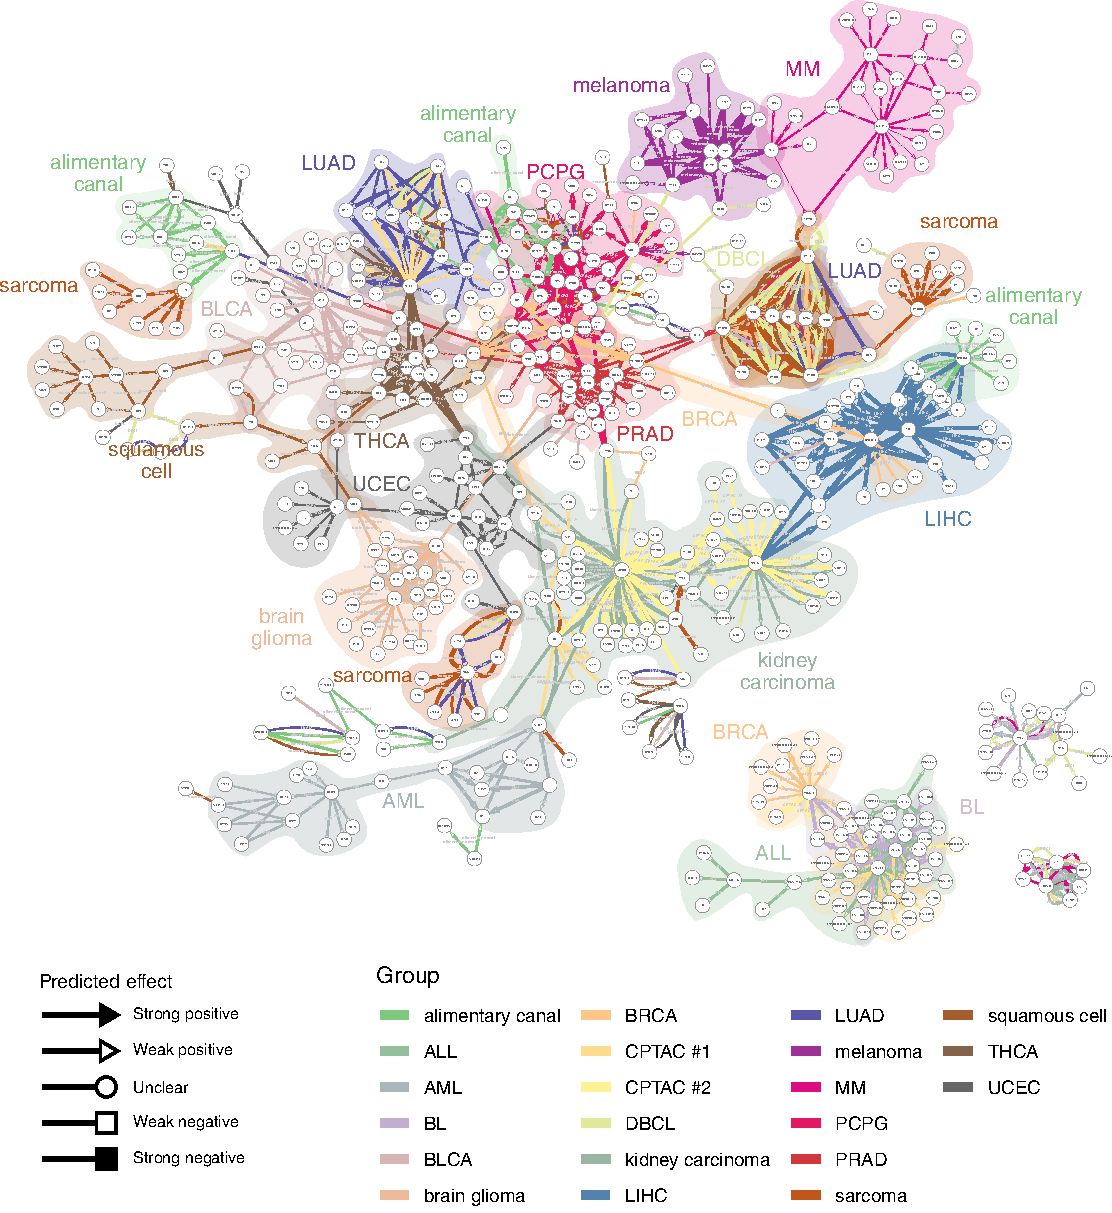
\includegraphics[width=\linewidth]{fig/tcga/grouped_interactions.pdf} 
	\caption{
		A
	}
	\label{fig:tcga}
\end{figure}


\section{Discussion}

\section{Methods}

\clearpage
\section{References}
\printbibliography[heading=none]
